\section{Results}
\FloatBarrier

\subsection{Clean-image detection across datasets}
Table~\ref{tab:detection} reports clean-image performance at the fixed decision threshold. ROC-AUC decreased from Columbia Uncompressed to CASIA v1 and COVERAGE for both frozen models. TruFor's AUC was 0.9958, 0.9052 and 0.7675, respectively; MVSS-Net's was 0.9752, 0.8390 and 0.7385. Columbia therefore provides a comparatively favorable result for these checkpoints and should not be treated as a sufficient estimate of performance on the other datasets. The same ordering is not captured fully by AUC alone: at threshold 0.5, MVSS-Net's Columbia F1 was 0.7412 despite its AUC of 0.9752, reflecting 124 false positives among 183 authentic images.

\begin{table}[t]
\centering
\caption{Clean-image detection performance for the frozen models. F1 uses the fixed 0.5 image-score threshold; ROC-AUC is threshold-free.}
\label{tab:detection}
\small
\begin{tabular}{llrrr}
\toprule
Dataset & Model & Detection $n$ & ROC-AUC & F1 \\
\midrule
Columbia Uncompressed & TruFor & 363 & 0.9958 & 0.9861 \\
 & MVSS-Net & 363 & 0.9752 & 0.7412 \\
CASIA v1 corrected & TruFor & 1,721 & 0.9052 & 0.7926 \\
 & MVSS-Net & 1,721 & 0.8390 & 0.7492 \\
COVERAGE corrected & TruFor & 200 & 0.7675 & 0.5811 \\
 & MVSS-Net & 200 & 0.7385 & 0.6714 \\
\bottomrule
\end{tabular}
\end{table}

\begin{figure}[t]
\centering
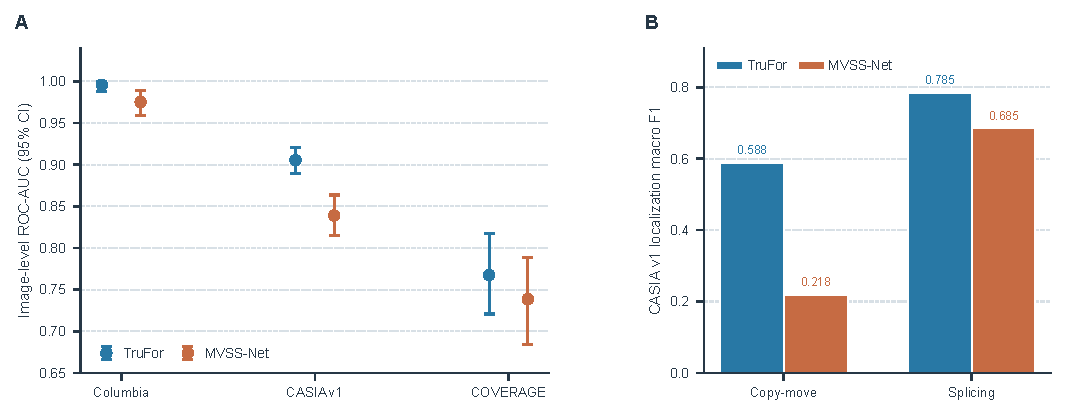
\includegraphics[width=\linewidth]{reports/figures/cross_dataset_comparison.pdf}
\caption{Cross-dataset detection and manipulation-type localization results. (A) Image-level ROC-AUC with dataset-specific 95\% bootstrap confidence intervals for Columbia Uncompressed ($n=363$), corrected CASIA v1 ($n=1{,}721$) and corrected COVERAGE ($n=200$). (B) CASIA v1 macro localization F1 by manipulation type, computed on valid reference masks (copy-move $n=459$; splicing $n=461$). Columbia confidence intervals use source-group bootstrap; CASIA and COVERAGE intervals use their prespecified bootstrap procedures.}
\label{fig:cross-dataset}
\end{figure}

On CASIA v1, the paired model difference in ROC-AUC was 0.0662 in favor of TruFor (95\% bootstrap CI 0.0462--0.0864; $p=0.0004$); the detection F1 difference was 0.0435 (0.0172--0.0695; $p=0.0012$). These paired comparisons are specific to the corrected CASIA v1 test bundle. Because the MVSS-Net checkpoint was trained on CASIAv2 and the local CASIA v1 bundle is not the authors' CASIAv1plus construction, possible authentic-content overlap remains a qualification on this comparison.

\subsection{Localization and manipulation-type differences}
Table~\ref{tab:localization} reports macro F1 on valid masks. Columbia results are listed for completeness but refer to overlap with its blue splice-boundary/camera-region annotation, not a complete tampered-area mask. CASIA and COVERAGE use manipulated-region references and are therefore the primary mask-localization comparisons. On CASIA, TruFor obtained higher overall F1 than MVSS-Net (0.6868 versus 0.4518); the paired difference was 0.2351 (95\% CI 0.2084--0.2614; $p=0.0004$). Both models localized splicing better than copy-move: TruFor F1 was 0.7854 versus 0.5879, while MVSS-Net F1 was 0.6848 versus 0.2177. The model-level average thus conceals a manipulation-specific performance gap.

\begin{table}[t]
\centering
\caption{Macro localization F1 on dimension-aligned reference masks. Columbia uses a dataset-specific boundary/source-region reference and should not be interpreted as directly comparable to complete tampered-region masks.}
\label{tab:localization}
\small
\begin{tabular}{llrr}
\toprule
Dataset / stratum & Model & Valid images & Macro F1 \\
\midrule
Columbia boundary reference & TruFor & 180 & 0.2613 \\
 & MVSS-Net & 180 & 0.2491 \\
CASIA v1, all tampering & TruFor & 920 & 0.6868 \\
 & MVSS-Net & 920 & 0.4518 \\
CASIA v1, copy-move & TruFor & 459 & 0.5879 \\
 & MVSS-Net & 459 & 0.2177 \\
CASIA v1, splicing & TruFor & 461 & 0.7854 \\
 & MVSS-Net & 461 & 0.6848 \\
COVERAGE, copy-move & TruFor & 91 & 0.5555 \\
 & MVSS-Net & 91 & 0.4817 \\
\bottomrule
\end{tabular}
\end{table}

\subsection{Sensitivity to compression and resizing}
The full-image stress tests applied JPEG recompression and resize--restore transformations to all Columbia and CASIA v1 images while keeping model weights and the 0.5 threshold fixed. Table~\ref{tab:stress} summarizes the clean condition, JPEG quality 40 and resize-to-0.25 condition. Results were transformation- and dataset-dependent. For example, TruFor's CASIA AUC fell from 0.9052 on clean images to 0.5923 after resize-to-0.25, while its Columbia AUC fell from 0.9958 to 0.8845. At the fixed threshold, CASIA TruFor F1 fell to 0.1583 and 34.40\% of binary decisions changed after the stronger resize. MVSS-Net also showed reduced AUC under stronger resizing, although the magnitude and thresholded F1 pattern differed by dataset. This variability cautions against treating one perturbation or one threshold-free metric as a general robustness certificate.

\begin{table}[t]
\centering
\caption{Selected full-image stress-test results. Each cell reports ROC-AUC / fixed-threshold detection F1. Flip rate is the fraction of image-level decisions changed from the clean prediction under resize-to-0.25.}
\label{tab:stress}
\small
\begin{tabular}{llrrr}
\toprule
Dataset & Model & Clean & JPEG q40 & Resize 0.25$\times$ \\
\midrule
Columbia & TruFor & 0.9958 / 0.9861 & 0.9861 / 0.8633 & 0.8845 / 0.8187 \\
 & MVSS-Net & 0.9752 / 0.7412 & 0.9642 / 0.7332 & 0.9057 / 0.7397 \\
CASIA v1 & TruFor & 0.9052 / 0.7926 & 0.8009 / 0.6612 & 0.5923 / 0.1583 \\
 & MVSS-Net & 0.8390 / 0.7492 & 0.6421 / 0.4855 & 0.6871 / 0.5402 \\
\midrule
Dataset & Model & \multicolumn{3}{c}{Flip rate at resize 0.25$\times$} \\
\midrule
Columbia & TruFor & \multicolumn{3}{c}{17.91\%} \\
 & MVSS-Net & \multicolumn{3}{c}{15.15\%} \\
CASIA v1 & TruFor & \multicolumn{3}{c}{34.40\%} \\
 & MVSS-Net & \multicolumn{3}{c}{31.67\%} \\
\bottomrule
\end{tabular}
\end{table}

Full metrics for all four stress transformations, including JPEG quality 80 and resize-to-0.5, are provided in Supplementary Table~\ref{tab:stress-complete}.

\begin{figure}[t]
\centering
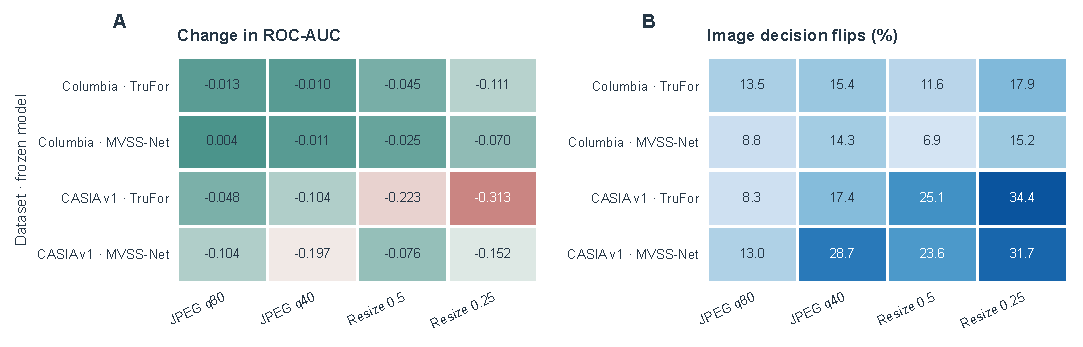
\includegraphics[width=\linewidth]{reports/figures/stress_sensitivity.pdf}
\caption{Sensitivity to controlled digital transformations. (A) Change in image-level ROC-AUC relative to the clean input for JPEG recompression (quality 80 and 40) and resize--restore (0.5 and 0.25 scale). (B) Image-level decision-flip rate relative to the clean prediction at the fixed 0.5 threshold. Rows identify dataset and frozen model; each Columbia condition includes 363 images and each CASIA v1 condition includes 1,721 images. Values are computed from the archived full-image stress summaries.}
\label{fig:stress}
\end{figure}

\subsection{Evidence completeness and independent replay}
For CASIA v1, one evidence record was generated for each of 1,721 images and two models (3,442 records total). ECR was 1.000 and ETR was 1.000. The independent-process replay sampled 90 cases per model, stratified evenly across authentic, copy-move and splicing classes. All source hashes matched and all 90 TruFor and 90 MVSS-Net cases reproduced both score and localization map within the absolute tolerance of $10^{-5}$; RSR and EGA were therefore 1.000 for each model. The Wilson 95\% interval was 0.959--1.000 for each 90/90 replay proportion. These results indicate complete records and deterministic replay in the tested environment. They do not show that every prediction is correct, that the model evidence is causally diagnostic, or that another machine will produce identical outputs.

The experiments also included handcrafted grayscale-statistics and ELA/logistic-regression baselines on a 73-image Columbia source-group test split. ELA reached ROC-AUC 0.8671 (95\% CI 0.6238--0.9701), compared with 0.8108 for grayscale statistics. These results use a smaller split; they are not paired against the frozen-model evaluation on 363 images.
